\documentclass{article}
\usepackage[utf8]{inputenc}
\usepackage{amsmath,graphicx,varioref,verbatim,amsfonts,geometry}
\usepackage[hidelinks]{hyperref}
\usepackage{listings}
\usepackage[T1]{fontenc}
\usepackage{mathtools}
\usepackage{textcomp}
\usepackage[english]{babel}
\usepackage{wrapfig}
\usepackage{fancyhdr}
\usepackage{enumitem}
\usepackage{xcolor}
\usepackage{lastpage}
\usepackage{graphicx}
\usepackage{matlab-prettifier}
\usepackage{filecontents}
\usepackage{underscore}
\usepackage{makecell}
\usepackage{caption}
\usepackage{subcaption}
\usepackage{siunitx}
\usepackage{mathrsfs}

\pagestyle{fancy}


%% Double underline 
\def\dubline#1{\underline{\underline{#1}}}

%% Matrix
\newcommand\SmallMatrix[1]{{%
		\arraycolsep=0.3\arraycolsep\ensuremath{\begin{pmatrix}#1\end{pmatrix}}}}
	
%% Codeinsert
\definecolor{listinggray}{gray}{0.9}
\definecolor{lbcolor}{rgb}{0.9,0.9,0.9}
\lstset{
	backgroundcolor=\color{lbcolor},
	tabsize=4,
	rulecolor=,
	language=python,
	basicstyle=\scriptsize,
	upquote=true,
	aboveskip={1.5\baselineskip},
	columns=fixed,
	numbers=left,
	showstringspaces=false,      
	extendedchars=true,
	breaklines=true,
	prebreak = \raisebox{0ex}[0ex][0ex]{\ensuremath{\hookleftarrow}},
	frame=single,
	showtabs=false,
	showspaces=false,
	showstringspaces=false,
	identifierstyle=\ttfamily,
	keywordstyle=\color[rgb]{0,0,1},
	commentstyle=\color[rgb]{0.133,0.545,0.133},
	stringstyle=\color[rgb]{0.627,0.126,0.941}
}
\newcounter{subproject}
\renewcommand{\thesubproject}{\alph{subproject}}
\newenvironment{subproj}{
	\begin{description}
		\item[\refstepcounter{subproject}(\thesubproject)]
	}{\end{description}}

\begin{document}
\title{IN3190 - Exam Preparation Questions H23\\
{\Large University of Oslo}}
\author{Daniel Tran}
\date{November 2023}
\fancyhead[L]{Should know to exam H23 - IN3190}
\fancyhead[C]{UiO}
\fancyhead[R]{Daniel Tran}
\cfoot{\thepage\ of \pageref{LastPage}}
\maketitle
\hypersetup{linkcolor=black}
\tableofcontents
\clearpage

\section{Essential Topics}
\subsection{Discrete time}
\subsubsection{Sine, cosine and exponential functions}

    Mathematical formula that establishes the fundamental relationship between the trigonometric functions and the complex exponential function. \newline
    Euler's formula states that for any real number $x$:
    \begin{equation}
        e^{ix} = \cos(x) + i\sin(x)
    \end{equation}
    When $x = \pi$, Euler's formula yields Euler's identity:
    \begin{equation}
        e^{i\pi} + 1 = 0
    \end{equation}
\subsubsection{Elementary discrete signals}
\paragraph{Unit impulse} %Spør gruppelærer om plot fra forelesning
Also known as the dirac delta function.
\begin{equation}
    \delta[n] = \begin{cases}
        1, & n = 0 \\
        0, & n \neq 0
    \end{cases}
    \hspace*{20pt}\text{may also be written as:}
    \hspace*{20pt} \delta[n] = u[n] - u[n-1]
\end{equation}

\begin{figure}[h!]
    \centering
    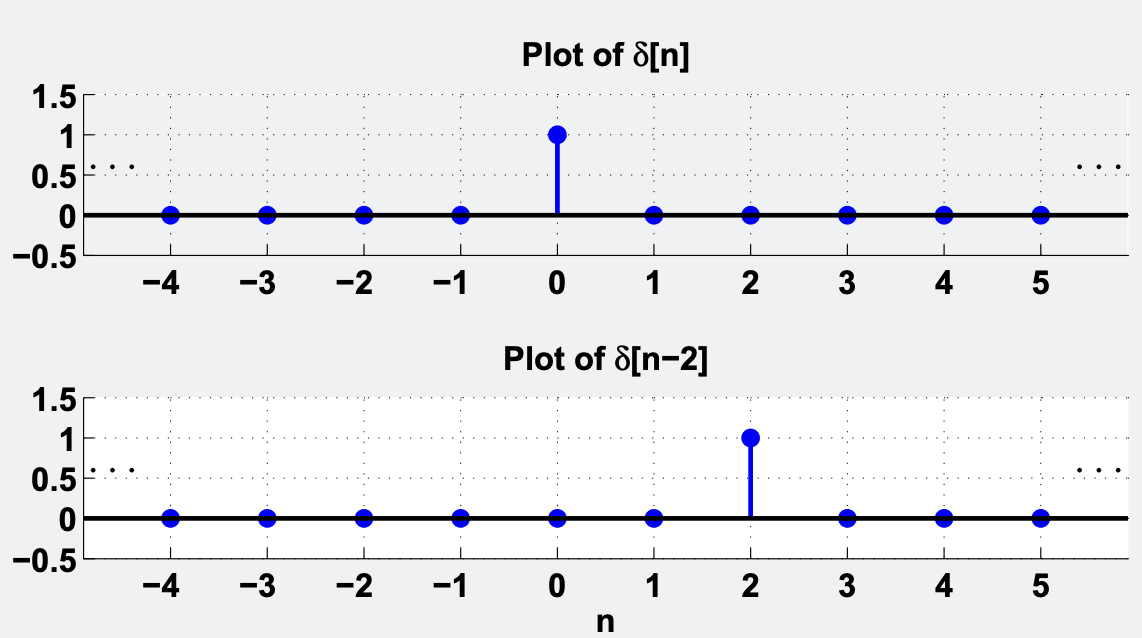
\includegraphics[width=0.5\textwidth]{figures/Discrete time/unit_impulse.png}
    \caption{Unit impulse}
    \label{fig:unit_impulse}
\end{figure}

\paragraph{Step function}
Also known as unit step, unit step function or heaviside function. The value which is zero for negative arguments and one for positive arguments.
\begin{equation}
    u[n] = \begin{cases}
        1, & n \geq 0 \\
        0, & n < 0
    \end{cases}
    \hspace*{20pt}\text{may also be written as:}
    \hspace*{20pt} u[n] = \sum_{k=0}^{\infty} \delta[n-k]
\end{equation}
\begin{figure}[h!]
    \centering
    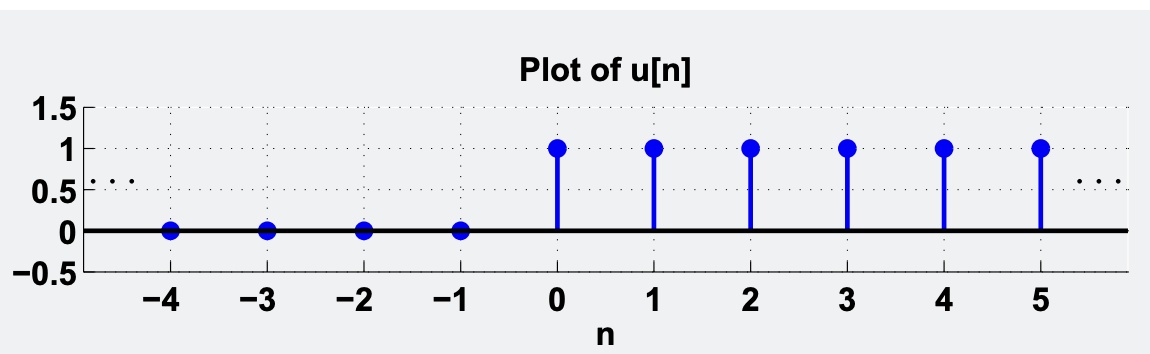
\includegraphics[width=0.5\textwidth]{figures/Discrete time/unit_step_function.png}
    \caption{Unit step function}
    \label{fig:unit_step}
\end{figure}

\newpage
\paragraph{Ramp function}
Also known as the unit-ramp or unit ramp function. Graph shaped like a ramp.
\begin{equation}
u_r[n] = \begin{cases}
    n, & n \geq 0 \\
    0, & n < 0
\end{cases}
\end{equation}
\begin{figure}[h!]
    \centering
    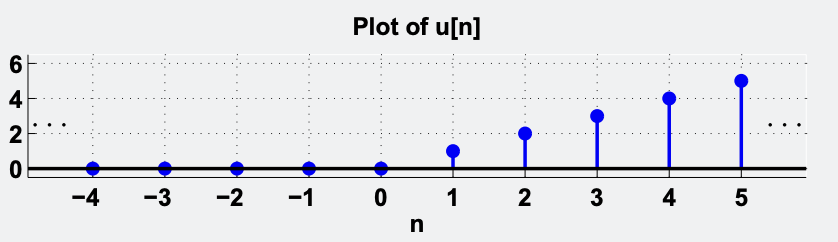
\includegraphics[width=0.5\textwidth]{figures/Discrete time/unit_ramp_function.png}
    \caption{Unit ramp function}
    \label{fig:unit_ramp}
\end{figure}

\paragraph{Periodic sequences} 
$x[n]$ is periodic if and only if $x[n] = x[n+N]$
\begin{itemize}
    \item \textbf{Fundamental period}: 
    \newline Smallest positive integer N which fulfills the relation above
    \item \textbf{Sinusoidal sequences}: 
    \newline $x[n] = A\cos(\omega_0n + \phi)$, where 
    \begin{itemize}
        \item $A$ is amplitude,
        \item $\omega_0$ is the angular frequency
        \item and $\phi$ is the phase of $x[n]$.
    \end{itemize} 
    $x[n]$ is periodic if and only if $\omega_0N = 2\pi k$, for N and k as positive integers.
\end{itemize}

\begin{figure}[h!]
    \centering
    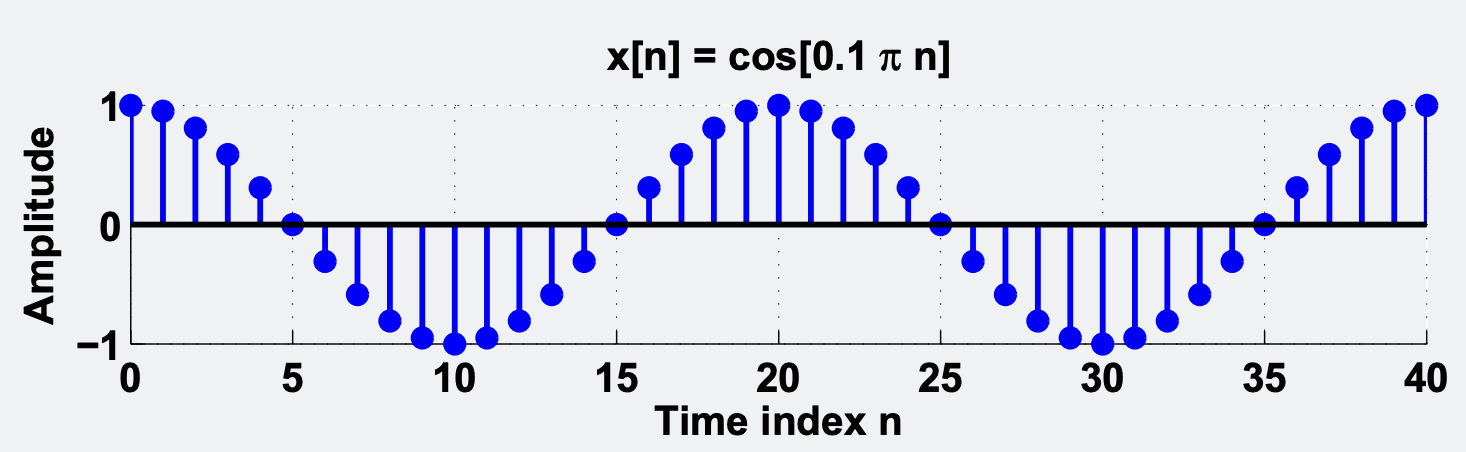
\includegraphics[width=0.5\textwidth]{figures/Discrete time/sinusoidal_sequences.png}
    \caption{Sinusoidal sequences}
    \label{fig:Sinusoidal_sequence}
\end{figure}

\subsubsection{LTI systems, including characteristics via the transformation between input and output}
\paragraph{Linearity:} The relationship between the input $x(t)$ and the output $y(t)$, both being regarded as functions. If $a$ is a constant then the system output to $ax(t)$ is $ay(t)$. Linear system if and only if it $H\{\cdot\}$ is both additive and homogeneous, in other words: If it fulfills the superposition principle. That is:
\begin{equation}
    H\{ax_1(t)+bx_x(t)\} = aH\{x_1(t)\} + bH\{x_2(t)\}
\end{equation}

\paragraph{Time-invariance:} 
A linear system is time-invariant or shift-invariant means that wether we apply an input to the system now or T seconds from now, the output will be identical except for a time delay of S seconds. In other words, if $y(t)$ is the output of a system with a input $x(t)$, then the output of the system with input $x(t-T)$ is $y(t-T)$. The system is invariant becasue the output does not depend on the particular time at which the input is applied.
\\
\\
The fundamental result in LTI system theory is that any LTI system can be characterized entirely by a single function called the system's impulse response $h(t)$. The output of the system $y(t)$ is simply the convolution of the input to the system $x(t)$ with the systems's impulse response $h(t)$.
\\
\\
LTI system can also be characterized in the frequency domain by the system's transfer function $H(s)$, which is the Laplace transform of the system's impulse response $h(t)$. Or Z-transform in the case of discrete time systems.
\begin{figure}[h!]
    \centering
    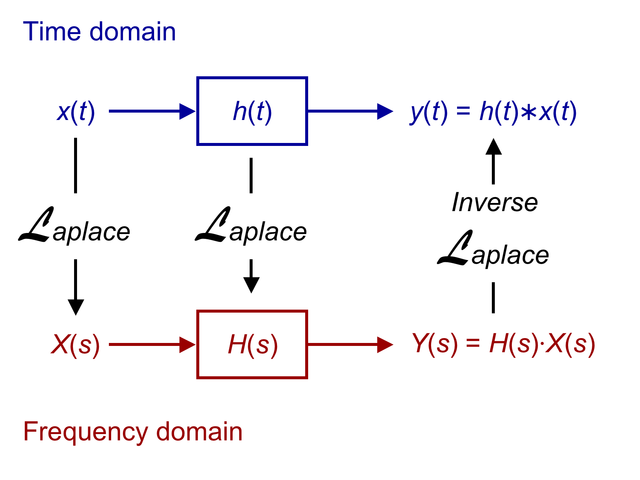
\includegraphics[width=0.5\textwidth]{figures/Discrete time/LTI_time_freq_domain.png}
    \caption{Relationship between the time domain and the frequency domain}
    \label{fig:lti_relationship}
\end{figure}

\subsection{Z-transform}

\subsection{Frequency analysis and DFT}

\subsection{Filter design}

\subsection{Sampling and reconstruction}

\section{Additional Topics}
\subsection{Discrete time}
\subsubsection{Symmetrical signals}

\subsection{LTI systems and characteristics}

\subsection{Convolution and correlation}

\subsection{Z-transform}

\subsection{Frequency analysis and DFT}

\subsection{Filter design}

\subsection{Sampling and reconstruction}
\end{document}